\def\year{2015}
%File: formatting-instruction.tex
\documentclass[letterpaper]{article}
\usepackage{aaai}
\usepackage{times}
\usepackage{helvet}
\usepackage{courier}
\usepackage{graphicx}
\frenchspacing
\setlength{\pdfpagewidth}{8.5in}
\setlength{\pdfpageheight}{11in}
\pdfinfo{
/Title (Affective Motivational Collaboration Theory)
/Author (Put All Your Authors Here, Separated by Commas)}
\setcounter{secnumdepth}{0}  

\usepackage{atbegshi,picture}
%\usepackage{lipsum}

% \AtBeginShipout{\AtBeginShipoutUpperLeft{%
%   \put(\dimexpr\paperwidth-6.5cm\relax,-1.5cm){\makebox[0pt][r]{\framebox{SUBMITTED
%   TO AAAI FALL SYMPOSIUM 2015. PLEASE DO NOT REDISTRIBUTE.}}}%
% }}

 \begin{document}
% The file aaai.sty is the style file for AAAI Press 
% proceedings, working notes, and technical reports.
%
\title{Affective Motivational Collaboration Theory}
\author{Mahni Shayganfar, Charles Rich, Candace L. Sidner\\
Worcester Polytechnic Institute\\
Computer Science Department\\
100 Institute Rd, Worcester, MA 01609\\
+1-508-847-4492\\
http://users.wpi.edu/{\raise.17ex\hbox{$\scriptstyle\sim$}}mshayganfar/\\
mshayganfar $|$ rich $|$ sidner@wpi.edu\\
}
\maketitle
\begin{abstract}
\begin{quote}
We investigate the mutual influence of affective and collaboration processes in
a cognitive theory to support the interaction between humans and robots or
virtual agents. We have developed new algorithms for some of these processes, as
well as a new overall computational model for implementing collaborative robots
and agents. We build primarily on the \textit{cognitive appraisal} theory of
emotions and the \textit{SharedPlans} theory of collaboration to investigate the
structure and fundamental processes of affect in a collaboration context. As
part of this work, we also address a deficiency in existing cognitive models by
accounting for the influence of motivation on collaborative behaviors, such as
overcoming an impasse. This motivation mechanism uses the results of cognitive
appraisal to dynamically form new intentions related to the collaboration
structure.
\end{quote}
\end{abstract}

\vspace*{-1mm}
An important aspect of the sociability of robots and agents is their ability to
collaborate with humans in the same environment. There are many challenges in
achieving collaboration between robots/agents and humans in the same
environment. One important issue is to understand what makes a collaboration
effective. One's cognitive processes and the ability to understand the
collaborative environment impact the effectiveness of a collaboration. Examples
of cognitive capabilities that support the effectiveness of collaboration
include: a) perceiving one's own internal states and b) communicating them, c)
coordinating personal and group behaviors, d) identifying self and mutual
interests, e) recognizing the accountability of private and shared goals, f)
selecting appropriate actions with respect to events, and g) engaging others in
collaboration.

Thus, it is crucial to investigate the cognitive processes involved in a
collaboration in the context of a cognitive architecture. There are several
well-developed cognitive architectures, e.g., Soar \cite{laird:soar} and ACT-R
\cite{anderson:act-r}, each with different approaches to defining the basic
cognitive and perceptual operations. There have also been efforts to integrate
affect into these architectures \cite{marinier:behavior-emotion}. In general,
however, these cognitive architectures do not focus on processes to specifically
produce affect-regulated goal-driven collaborative behaviors. At the same time,
existing collaboration theories, e.g. SharedPlans theory
\cite{grosz:plans-discourse}, Joint Intentions \cite{cohen:teamwork}, and STEAM
\cite{tambe:flexible-teamwork}, focus on describing the structure of a
collaboration in terms of mental states, e.g., mutual beliefs or intentions.
However, they do not describe the associated processes, their relationships, and
their influences on each other. In contrast, in \textit{Affective Motivational
Collaboration Theory}, we are interested to investigate and explain major
processes, including affective and motivational processes, having an impact on
the collaboration structure. Our contribution, generally speaking, is to
synthesize prior work on motivation, appraisal and collaboration, and thus to
provide a new theory which describes the prominent affect-regulated goal-driven
processes in a dyadic collaboration.

\vspace*{-3mm}
\section{Affect and Collaboration}

Collaboration is a coordinated activity in which the participants work jointly
to satisfy a shared goal \cite{grosz:plans-discourse}. There are many important
unanswered questions about the involvement of an individual's cognitive
abilities during collaboration. Some of these questions are related to the
dynamics of collaboration, as well as the underlying mechanisms and processes.
For instance, a general mechanism has yet to be developed that allows an agent
to initiate proactive collaborative behaviors when it faces a blocked task.
There is also a lack of a general mechanism that, in the event of a task
failure, allows an agent to consider the collaborator's anticipated mental
states and emotions, while managing its own internal goals and the
collaboration's shared goal. There are also other questions about the components
involved in these processes at the cognitive level, such as the processes that
are involved for evaluative, regulatory or motivative purposes.

Emotions have a key role in influencing the cognitive processes involved in
social interaction and collaboration. Emotion processing and decision-making are
integral aspects of daily life and maintain their prominence during social
interaction and collaboration. However, researchers' understanding of the
interaction between emotions and collaborative behaviors is limited. We believe
that the evaluative role of emotions, as a part of cognitive processes, helps an
agent to perform appropriate behaviors during a collaboration. To work jointly
in a coordinated activity, participants (collaborators) act based on their own
understanding of the world and the anticipated mental states of the counterpart;
this understanding is reflected in their collaborative behaviors. Emotions are
pivotal in the collaboration context, since their regulatory and motivational
roles enhance an individual's autonomy and adaptation as well as his/her
coordination and communication competencies in a dynamic, uncertain and
resource-limited environment.

\vspace*{-1mm}
\begin{figure}[tbh]
  \centering
  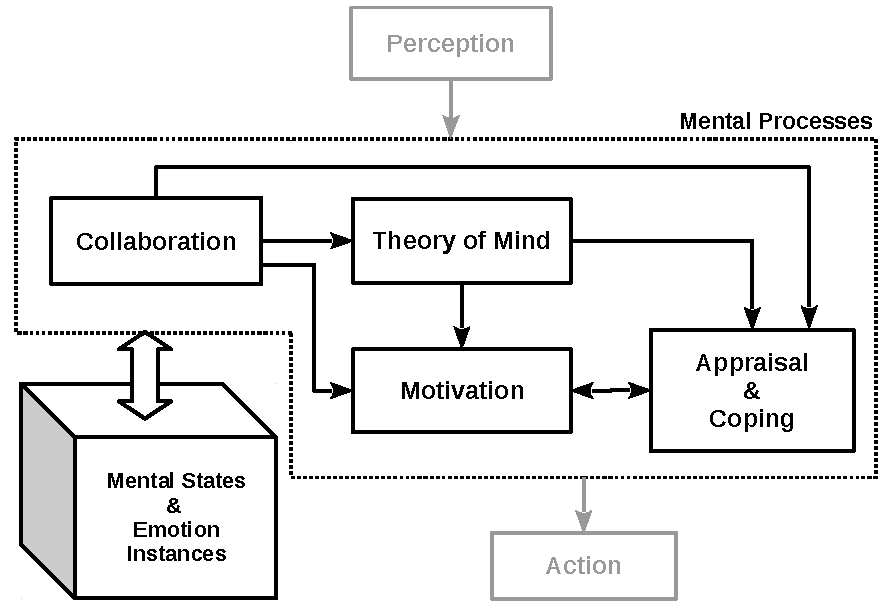
\includegraphics[width=0.474\textwidth]{figure/theory-general-croped.pdf}
  \caption{{\fontsize{8.5}{9}\selectfont Computational framework based on
  Affective Motivational Collaboration Theory (arrows indicate primary
  influences between mechanisms).}}
  \label{fig:cpm}
\end{figure}

\vspace*{-7mm}
\section{Affective Motivational Collaboration Theory}

We are building Affective Motivational Collaboration Theory on the foundations
of the \textit{SharedPlans} theory of collaboration \cite{grosz:plans-discourse}
and the \textit{cognitive appraisal} theory of emotions
\cite{gratch:domain-independent}. Affective Motivational Collaboration Theory is
about the interpretation and prediction of observable behaviors in a dyadic
collaborative interaction. The theory focuses on the processes regulated by
emotional states. The observable behaviors represent the outcome of reactive and
deliberative processes related to the interpretation of the self's relationship
to the collaborative environment. Affective Motivational Collaboration Theory
aims to explain both rapid emotional reactions to events as well as slower, more
deliberative responses. The reactive and deliberative processes are triggered by
two types of events: \textit{external} events, such as the other's
\textit{utterances} and \textit{primitive actions}, and \textit{internal}
events, comprising changes in the self's mental states, such as belief formation
and emotional changes. Affective Motivational Collaboration Theory explains how
emotions regulate the underlying processes when these events occur during
collaboration. This theory elucidates the role of motives as goal-driven
emotion-regulated constructs with which an agent can form new intentions to cope
with internal and external events. Our focus is on the mechanisms depicted as
mental processes in Figure \ref{fig:cpm} along with the mental states.

The \textit{Mental States} includes self's (robot's) beliefs, intentions,
motives, goals and emotion instances as well as the anticipated Mental States of
the other (human). The \textit{Collaboration} mechanism maintains constraints on
actions, including task states and the ordering of tasks. The
\textit{Collaboration} mechanism also provides processes to update and monitor
the shared plan. The \textit{Appraisal} mechanism is responsible for evaluating
changes in the self's Mental States, the anticipated Mental States of the other,
and the state of the collaboration environment. The \textit{Coping} mechanism
provides the self with different coping strategies associated with changes in
the self's mental states with respect to the state of the collaboration. The
\textit{Motivation} mechanism operates whenever the self a) requires a new
motive to overcome an internal impasse in an ongoing task, or b) wants to
provide an external motive to the other when the other faces a problem in a
task. The \textit{Theory of Mind} mechanism is the mechanism that infers a model
of the other's anticipated mental state. The self progressively updates this
model during the collaboration.

\vspace*{-3mm}
\section{Conclusion}

Current computational theories for human-robot collaboration specify the
structure of collaborative activities, but are weak on the underlying processes
that generate and maintain these structures. Emotions, due to their regulatory,
evaluative, communicative, and motivative functions can play a key role in the
underlying processes of collaboration. We are developing a new computational
theory, called Affective Motivational Collaboration Theory, that combines
affective processes, such as appraisal and coping, with collaboration processes,
such as planning, in a single unified framework.

The theoretical part of our computational architecture is primarily
investigated. The major required mechanisms involved in our computational
framework are known. We have implemented a few hypothetical collaboration
examples. We have used JESS (Java Expert System Shell) language to simulate some
of the crucial processes in our framework and speculate about the relationships
between different mechanisms and their underlying processes. We have recently
developed algorithms to compute four appraisal variables, i.e.,
\textit{relevance, desirability, expectedness} and \textit{controllability}
using collaboration's structure (\textit{https://github.com/mshayganfar}
includes recent developments). We conduct a study to compare the results of
human subjects' evaluation of some events and our agent's appraisals. We will
develop and integrate the Motivation mechanism into our framework in the next
step.

%This work was supported in part by the National Science Foundation under award
%IIS-1012083.

\vspace*{-3mm}

\bibliography{mshayganfar.bib}
\bibliographystyle{aaai}

\end{document}
